\subsection{Burnside's Lemma}

Let $G$ be a group that acts on a set $X$. The Burnside Lemma states that the number of distinct orbits is equal to the average number of points fixed by an element of G.
$$T = \frac{1}{|G|} \sum_{g \in G} |\texttt{fix}(g)|$$
Where a orbit $\texttt{orb}(x)$ is defined as
$$\texttt{orb}(x) = \{y \in X : \exists g \in G \ gx = y \}$$
and $\texttt{fix}(g)$ is the set of elements in $X$ fixed by $g$
$$\texttt{fix}(g) = \{x \in X : gx = x\}$$

\textbf{Example:} With $k$ distinct types of beads how many distinct necklaces of size $n$ can be made? Considering that two necklaces are equal if the rotation of one gives the other.

\begin{center}
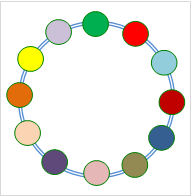
\includegraphics[scale=.6, keepaspectratio]{../theoretical/img/Burnside.png}
\end{center}

\begin{align*}
T &= \frac{1}{n+1} \sum_{i=0}^{n}k^{gcd(i, n)} & T &= \frac{1}{n} \sum_{i=0}^{n-1}k^{gcd(i, n)}
\end{align*}
